\documentclass[a4paper]{exam}

\usepackage{amsmath,amssymb, amsthm}
\usepackage{geometry}
\usepackage{graphicx}
\usepackage{hyperref}
\usepackage{xcolor}
\usepackage{wasysym}

\usepackage{tikz}
\usepackage{tikz-qtree}

\usepackage{scalerel}

\newcommand{\X}{\scalerel*{
\includegraphics{Annihilus.png}}{\mathbf{0}}}



\newtheorem{definition}{Definition}
\newtheorem{theorem}{Theorem}

\title{Weekly Challenge 02: Deterministic Finite Automata}
\author{Hassan Akhter (ha10609)}
\date{Fall 2026}

\boxedpoints


 \printanswers % Uncomment this line

\begin{document}
\maketitle


\begin{questions}


	\question
	For a language $L \subseteq \Sigma^*$, the $\X$ operator is defined as follows: $\X(L) = \{w \in \Sigma^*\mid w \not\in L\}$.

	Consider the language $L$ of strings of form $0^n1^m$ for $n,m \in \mathbb{Z}^+$.
	\begin{parts}
		\part Define $\X(L)$, and construct a FSM (DFA) for $\X(L)$.
		\begin{solution}
			% Enter your solution here 
      \\
			$\X(L) = \{w \in \Sigma^* \mid w \in {0,1}^*$ w not in form $0^n1^m$ for n,m in Z \\
      we can draw the DFA for L, then invert the accepting states to get $\X(L)$
			\begin{center}
				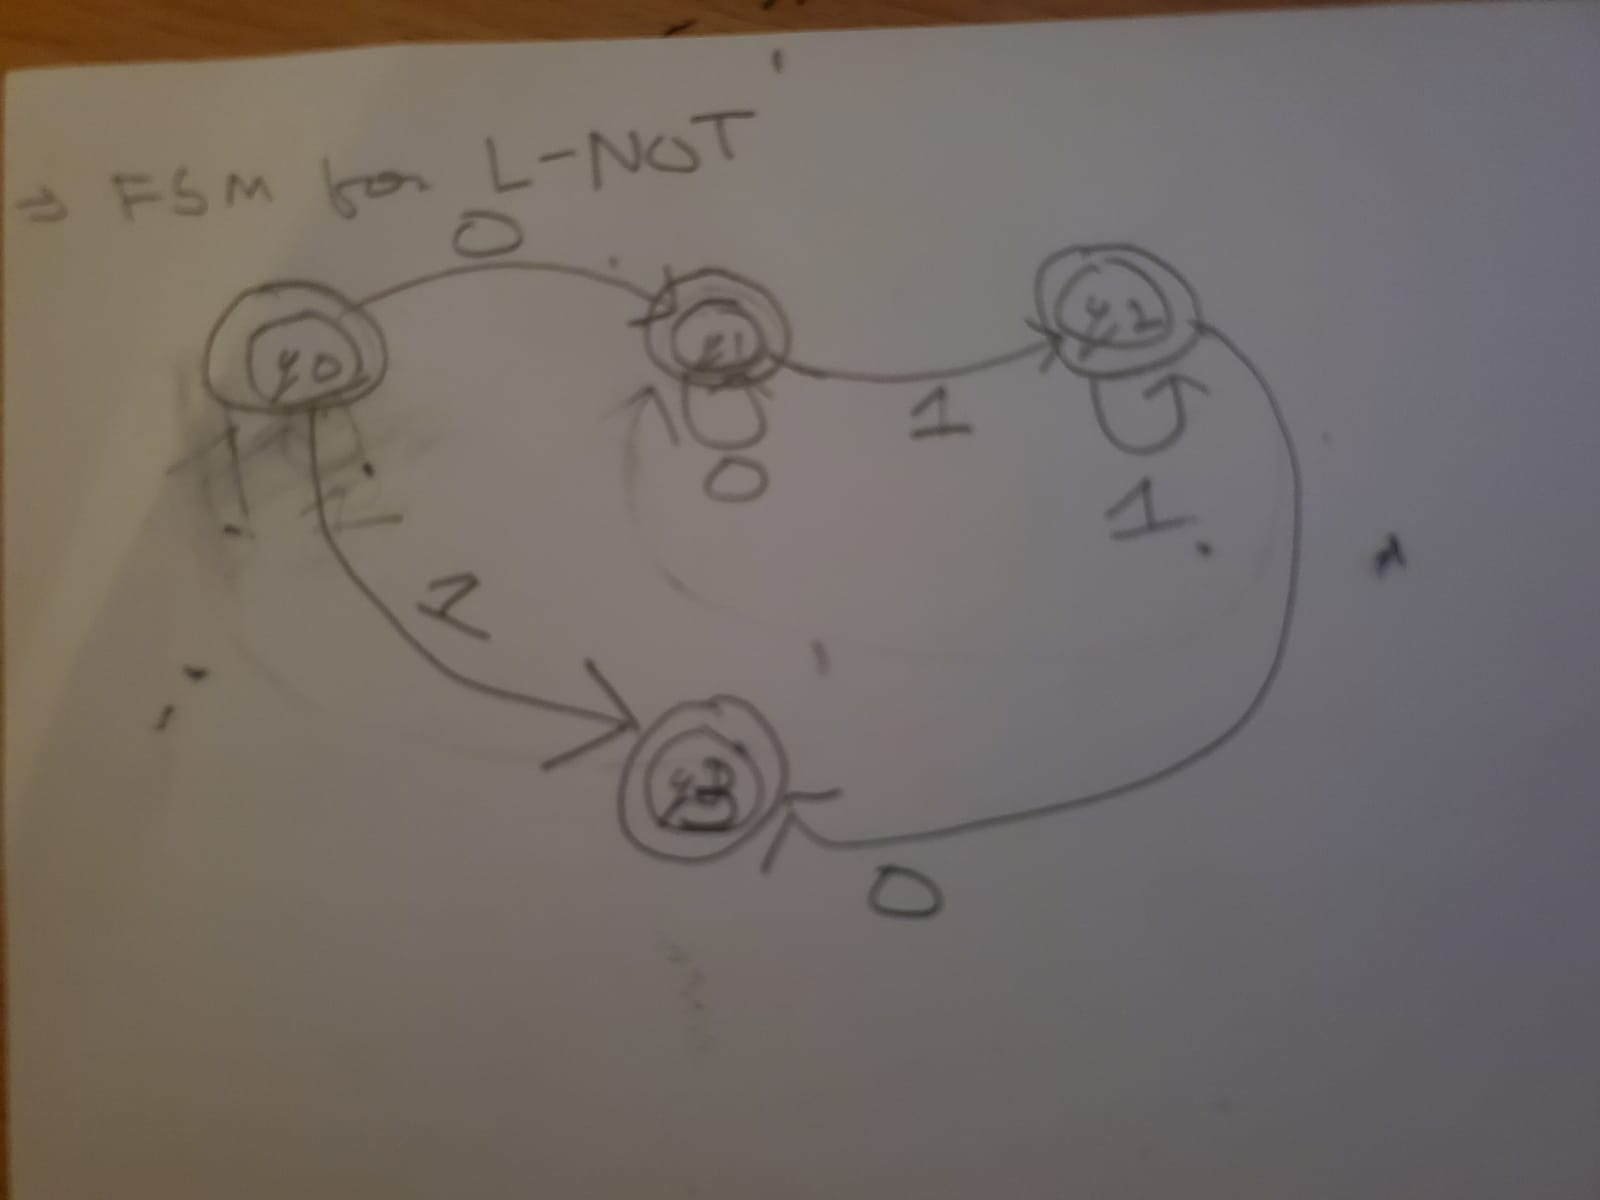
\includegraphics[width=0.95\textwidth]{./WhatsApp Image 2026-09-10 at 9.44.28 PM.jpeg}

				DFA
			\end{center}


		\end{solution}

		\part Prove or disprove the following claim: If a language $L \subseteq \Sigma^*$ is regular then $\X(L)$ is also regular.
		\begin{solution}
			% Enter your solution here
      \\
			If $L$ is a regular DFA defined $(Q, \Sigma, \delta, q_0, F)$, then there exists another DFA $L'$ such: \\
			$L' = (Q, \Sigma, \delta, q_0, Q \setminus F)$ \\
      This state accepts all states that are complement of L, as its accepting states are the not in set $F$ of the accepting states of L with other definitions identical. \\
      Therefore, $w \in L' \iff \delta(q_0, w) \in Q \setminus F$  \\
		\end{solution}
	\end{parts}


\end{questions}
\end{document}

%%% Local Variables:
%%% mode: latex
%%% TeX-master: t
%%% End:



